\documentclass[12pt,a4paper]{article}

\usepackage[portuguese]{babel}
\usepackage[utf8]{inputenc}
\usepackage[T1]{fontenc}
\usepackage{amsmath}
\usepackage{hyperref}
\usepackage{graphicx}

\author{Gabriel Tomé Silveira}
\title{\textbf{Segunda lista de exercícios}}

\begin{document}
\maketitle
	\pagebreak

	\section{Problema 1}
	\subsection{1a)}

	$$ F(k)=\frac{1}{2\pi}\int_{-\infty}^{\infty} s(x) e^{-ikx}dx $$
	\\
	\subsection{2a)}
	\begin{equation}
		\label{eq:n711}
		\begin{cases}
			\frac{dx}{dt} = \sigma(y-x)\\
			\frac{dy}{dt} = x(-z)-y\\
			\frac{dz}{dt} = xy-\beta z\\
		\end{cases}
	\end{equation}

	\subsection{Problema 3}
	\begin{figure}[!htb]
		\centering
		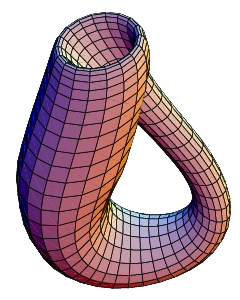
\includegraphics[scale=0.8]{KleinBottle-01}

	\end{figure}


\end{document}
%%% Local Variables:
%%% mode: latex
%%% TeX-master: t
%%% End:
